\documentclass[ignorenonframetext, professionalfonts, hyperref={pdftex, unicode}]{beamer}

\usetheme{Copenhagen}
\usecolortheme{wolverine}

%Packages to be included
%\usepackage{graphicx}

\usepackage[russian]{babel}
\usepackage[utf8]{inputenc}
\usepackage[T1]{fontenc}

%%\usepackage[orientation=landscape, size=custom, width=16, height=9.75, scale=0.5]{beamerposter}

\usepackage{textcomp}

\usepackage{beamerthemesplit}

\usepackage{ulem}

\usepackage{verbatim}

\usepackage{ucs}


\usepackage{listings}
\lstloadlanguages{bash}

\lstset{escapechar=`,
	extendedchars=false,
	language=sh,
	frame=single,
	tabsize=2, 
	columns=fullflexible, 
%	basicstyle=\scriptsize,
	keywordstyle=\color{blue}, 
	commentstyle=\itshape\color{brown},
%	identifierstyle=\ttfamily, 
	stringstyle=\mdseries\color{green}, 
	showstringspaces=false, 
	numbers=left, 
	numberstyle=\tiny, 
	breaklines=true, 
	inputencoding=utf8,
	keepspaces=true,
	morekeywords={u\_short, u\_char, u\_long, in\_addr}
	}

\definecolor{darkgreen}{cmyk}{0.7, 0, 1, 0.5}

\lstdefinelanguage{diff}
{
    morekeywords={+, -},
    sensitive=false,
    morecomment=[l]{//},
    morecomment=[s]{/*}{*/},
    morecomment=[l][\color{darkgreen}]{+},
    morecomment=[l][\color{red}]{-},
    morestring=[b]",
}

\author[Epam]{{\bf Epam}\\Low Level Programming Department}

%\institution[EPAM]{EPAM}
%\logo{\includegraphics[width=1cm]{logo.png}}

\title{Введение в GNU/Linux\\Командная строка}

\begin{document}
\begin{frame}
 \frametitle{}
 \titlepage
\end{frame}

\section{Принципы проектирования переносимых программ}
\mode<all>{\begin{frame}{Главные ориентиры}
	\begin{itemize}
		\item кроссплатформенная переносимость
		\item открытые стандарты
	\end{itemize}
\end{frame}

\begin{frame}{Немного цитат}
Дуг Макилрой, изобретатель каналов <<pipes>>, сформулировал несколько постулатов,применимых для разработки ПО:
\pause
	\begin{itemize}
		\item пишите программы,  которые выполняют одну функцию и делают это хорошо;
			\pause
		\item пишите программы,  которые будут работать вместе;
			\pause
		\item пишите программы,  поддерживающие текстовые потоки,  поскольку они являются универсальным интерфейсом.
	\end{itemize}

\end{frame}


\begin{frame}{"Философия" UNIX}
	это {\bfseries не} философия,  а общие рекомендации по проектированию ПО,  накопленные сообществом программистов на опыте десятилетий разработок программ,  которые взаимодействуют друг с другом.
\end{frame}

\begin{frame}{1. Правило модульности}
	\begin{block}{Следует писать простые части,  связанные ясными интерфейсами.}
Единственным способом создания сложной программы,  не обреченной заранее на провал,  является сдерживание ее глобальной сложности.
	\end{block}
Т.е. построение программы из простых частей, соединенных четко определенными интерфейсами, 
так что большинство проблем являются локальными, 
и тогда можно рассчитывать на обновление одной из частей без разрушения целого.
\end{frame}

\begin{frame}{Размер кода и ошибки}
	\begin{center}
		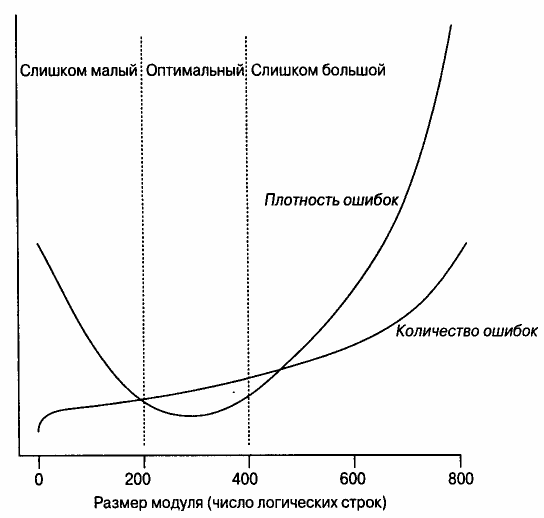
\includegraphics[width=200px]{../../slides/intro/errors_density-graph.png}
	\end{center}
\end{frame}

\begin{frame}{2. Правило ясности}
	\begin{block}{Ясность -- лучше чем мастерство.}
		Последующее обслуживание программы -- важная и дорогостоящая часть жизненного цикла программы.
	\end{block}
	\pause
Писать программы необходимо так,  как если бы вы знали,  что последующей поддержкой будет заниматься неуравновешенный псих с топором,  знающий ваш домашний адрес!
\end{frame}

\begin{frame}{3. Правило композиции}
	\begin{block}{Следует разрабатывать программы,  которые будут взаимодействовать с другими программами.}
		Если разрабатываемые программы не способны взаимодействовать друг с другом,  то очень трудно избежать создания сложных монолитных  программ.
	\end{block}
	Методы взаимодействия могут быть сильными и слабыми -- по возможности рекомендуется использовать слабые методы и текстовые форматы передачи данных.
\end{frame}

\begin{frame}{4. Правило разделения}
	\begin{block}{Следует отделять политику от механизма и интерфейсы от основных модулей (engine).}
		Примеры политики и механизма:\\
		вид GUI и операции отрисовки, клиент (front-end) -- сервер (back-end), сценарии и библиотеки и др.
	\end{block}
	При жесткой связи политики и механизма:
	\begin{itemize}
		\item политика становится негибкой и усложняется ее изменение;
		\item изменение политики имеет строгую тенденцию к дестабилизации механизмов.
	\end{itemize}
\end{frame}

\begin{frame}{5. Правило простоты}
	\begin{block}{Необходимо проектировать простые программы и <<добавлять сложность>> только там,  где это необходимо.}
	\end{block}
	Основные причины добавления сложности:
	\begin{itemize}
		\item человеческий фактор (часто -- желание <<выпендриться>>);
		\item проектные требования,  продиктованные текущей модой,  маркетингом или «левой пяткой заказчика»;
	\end{itemize}
\end{frame}

\begin{frame}{6. Правило расчетливости}
	\begin{block}{Пишите большие программы,  только если после демонстрации становится ясно,  что ничего другого не остается.}
		Под <<большими программами>> здесь понимаются программы с большим объемом кода и значительной внутренней сложностью.
	\end{block}
\end{frame}

\begin{frame}{7. Правило прозрачности}
	\begin{block}{Для того,  чтобы упростить проверку и отладку программы,  ее конструкция должна быть обозримой.}
		Программа {\itshape прозрачна}, если при ее минимальном изучении можно понять, что она делает и как.\\
		Программа {\itshape воспринимаема},  когда она имеет средства для мониторинга и отображения внутреннего состояния.
	\end{block}
	Необходимо использовать достаточно простые форматы входных и выходных данных.\\
	Интерфейс должен быть приспособлен для использования в отладочных сценариях.
\end{frame}

\begin{frame}{8. Правило устойчивости}
	\begin{block}{Устойчивость -- следствие	прозрачности и простоты.}
		Программа является {\itshape устойчивой},  когда она выполняет свои функции в неожиданных условиях,  которые выходят за рамки предположений разработчика,  как и в нормальных условиях.\\
		Программа является {\itshape простой},  если происходящее в ней не представляется сложным для восприятия человеком.
	\end{block}
	Один из способов организации -- модульность(простые блоки,  ясные интерфейсы)\\
	Следует избегать частных случаев!
\end{frame}

\begin{frame}{Пример неусточивого ПО}
	\begin{center}
		
\includegraphics[width=1\textwidth]{../../slides/intro/exploits_of_a_mom_rus.png}
	\end{center}
\end{frame}


\begin{frame}[fragile]{Пример <<простой>> программы}
	\begin{center}
		\begin{verbatim}
+++++++++++++++++++++++++++++++++++++++++++++
+++++++++++++++++++++++++++.+++++++++++++++++
++++++++++++.+++++++..+++.-------------------
---------------------------------------------
---------------.+++++++++++++++++++++++++++++
++++++++++++++++++++++++++.++++++++++++++++++
++++++.+++.------.--------.------------------
---------------------------------------------
----.-----------------------.
		\end{verbatim}
	\end{center}
\end{frame}

\begin{frame}{9. Правило представления}
	\begin{block}{Знания следует оставлять в данных,  чтобы логика программы могла быть примитивной и устойчивой.}
		Даже простую логику бывает сложно проверить,  но даже сложные структуры данных являются довольно простыми для моделирования и анализа (например диаграмма 50 узлов дерева и блок-схема 50 строк кода)
	\end{block}
	Если можно выбирать между усложнением структуры данных и усложнением кода,  то лучше выбирать первое.\\
	Примеры: ascii,  генератор html-таблицы.
\end{frame}

\begin{frame}{10. Правило наименьшего удивления}
	\begin{block}{При проектировании интерфейсов всегда следует использовать наименее неожиданные элементы.}
		Необходимо учитывать характер предполагаемой аудитории и традиции платформы.
	\end{block}
	Оборотная сторона: следует избегать создания внешне похожих вещей,  слегка отличающихся в действительности,  поскольку {\itshape кажущаяся привычность порождает ложные ожидания}.
\end{frame}

\begin{frame}{11. Правило тишины}
	\begin{block}{Если программе нечего сказать,  то пусть лучше молчит.}
		Внимание и сосредоточенность пользователя -- ценный и ограниченный ресурс,  который требуется только в случае необходимости.
	\end{block}
	Важная информация не должна смешиваться с подробными сведениями о работе программы.
\end{frame}

\begin{frame}{12. Правило восстановления}
	\begin{block}{Когда программа завершается аварийно,  это должно происходить явно (шумно) и по возможности быстро.}
		Если программа не способна справиться с ошибкой,  то необходимо завершить ее работу так,  чтобы максимально упростить диагностику.
	\end{block}
	Для сетевых служб следует следовать рекомендации Постела:\\
	<<{\itshape Будьте либеральны к тому,  что принимаете,  и консервативны к тому,  что отправляете}>>
\end{frame}

\begin{frame}{13. Правило экономии}
	\begin{block}{Время программиста дорого -- поэтому задача экономии его времени более приоритетна,  по сравнению с экономией машинного времени.}
		Компьютер железный -- ему не скучно (с) программистская мудрость
	\end{block}
	Использование высокоуровневых языков и <<обучение>> машины выполнять больше низкоуровневой работы по программированию,  что приводит к правилу 14.
\end{frame}

\begin{frame}{14. Правило генерации}
	\begin{block}{Избегайте кодирования вручную; если есть возможность -- пишите программы для создания программ.}
		Использование генераторов кода оправданно,  когда они могут повысить уровень абстракции,  
		т.е. когда язык спецификации для генератора проще,  чем сгенерированный код,  
		и код впоследствии не потребует ручной доработки.
	\end{block}
	Примеры: грамматические и лексические анализаторы,  генераторы make-файлов,  построители GUI-интерфейсов.
\end{frame}

\begin{frame}{15. Правило оптимизации}
	\begin{block}{Сначала -- опытный образец,  потом -- оптимизирование.}
		Добейтесь стабильной работы,  только потом оптимизируйте.
	\end{block}
	\begin{block}{Керниган и Плоджер:}
		90\% актуальной и реальной функциональности лучше,  чем 100\% функциональности перспективной и сомнительной
	\end{block}
	\begin{block}{Кнут:}
		преждевременная оптимизация -- корень всех зол
	\end{block}
	\begin{block}{Кент Бек (экстремальное программирование):}
		заставьте программу работать,  заставьте работать ее верно,  а затем сделайте ее быстрой
	\end{block}
\end{frame}

\begin{frame}{16. Правило разнообразия}
	\begin{block}{Не следует доверять утверждениям о <<единственно правильном пути>>.}
		Никто не обладает умом,  достаточым для оптимизации всего или для предвидения всех возможных вариантов использования создаваемой программы.
	\end{block}
\end{frame}

\begin{frame}{17. Правило расширяемости}
	\begin{block}{Разрабатывайте для будущего. Оно наступит быстрее,  чем вы думаете.}
		При проектировании протоколов или форматов файлов следует делать их самоописательными,  для того,  чтобы их можно было расширить.
	\end{block}
	{\itshape Всегда},  следует либо включать номер версии,  либо составлять формат из самодостаточных,  
	самоописательных команд так,  чтобы можно было легко добавить новые директивы,  
	а старые удалить, <<не сбивая с толку>> код чтения формата.
\end{frame}

\begin{frame}{Все правила сразу}
	\begin{center}
	{\Huge\bfseries K.I.S.S.}

	Keep It Simple,  Stupid!
	\end{center}
\end{frame}


}

\section{Интерфейс командной строки}
\mode<all>{% Тема. Командная строка. 
% Показать примеры использования. Рассказать о преимуществах и недостатках в
% сравненни с графическим "оконным" интерфейсом. 
% Ознакомить с назначениме  эмулятора терминала и об реализациях.

\begin{frame}{Примеры использования командной строки}
	\begin{columns}
	\column{0.5\textwidth}
        \begin{itemize}
            \item чаты
            \item компьютерные игры Quake, DotA
            \item операционные системы
        \end{itemize}
	\column{0.5\textwidth}
	% insert picture of Quake 
    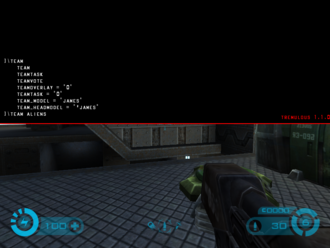
\includegraphics[height=0.4\textheight]{../../slides/cmdline/330px-Tremulous_console.png}
	\end{columns}
\end{frame}

\begin{frame}{Преимущества командной строки}
	\begin{itemize}
		\item Работа через сеть либо RS232
		\item Быстрый доступ к командам системы
		\item Легче отладка сообществом
		\item Легкость автоматизации
	\end{itemize}
\end{frame}

\begin{frame}{Недостатки командной строки}
	\begin{itemize}
		\item Oтсутствуют возможности обнаружения (discoverabililty)
		\item Необходимость изучения синтаксиса команд и запоминания сокращений.  (синтаксис может различаться)
		\item Без автодополнения, ввод длинных и содержащих спецсимволы параметров с клавиатуры может быть затруднительным
		\item Отсутствие «аналогового» ввода.
	\end{itemize}
\end{frame}

\begin{frame}{Эмуляторы терминала в графическом режиме}
	\begin{itemize}
		\item xterm
		\item rxvt
        \item gnome-terminal
        \item konsole
        \item Yakuake (Yet Another Kuake)
	\end{itemize}
\end{frame}
\note { 
Примеры приложений которые лучше выглядят в графическом режиме браузер,
редакторы видео и графики. Поэтому пользователь при работе, как правило,
совмещает оба интерфейса: использует графическое окружениe в сочетании с
интерфейсом командной строки. 
В графическом окружении интерфейса командной строки предоставляют приложения -
эмуляторы терминала. 
реализации - для графической системы X Window xterm, rxvt. Для GNOME
gnome-terminal, для KDE konsole, Yakuake (Yet Another Kuake выезжает по нажатии
тильды ~ как Quake)  
Дополнительные замечания:
Терминал - устройство для ввода вывода информации, уже устарел.
Графические приложения можно запускать из командной строки. 
}
}

\section{ Командная оболочка(shell) }
\begin{frame}
\frametitle{}
 \begin{center}
   {\Large Командная оболочка(shell) }
 \end{center}
\end{frame}

\mode<all>{\begin{frame}[fragile]{Определение(не совсем формальное)}
	\textbf{Shell} -- приложение, обеспечивающее выполнение других приложений и их взаимодействие, а также представляющая услуги командной строки. 
	\begin{center}
	 или
	\end{center}
	\textbf{Shell} -- приложение, обеспечивающее доступ к основным функциям ядра.

	\pause
	\vspace{0.5in}
	Пример shell из Windows-world -- cmd.exe
	\vspace{0.5in}

	Минимальный дистрибутив Linux -- ядро + shell 

\end{frame}

\begin{frame}[fragile]{Основные типы shell в Unix}
  \begin{itemize}
    \item Bourne shell совместимые
      \begin{itemize}
        \item \textbf{sh} исходная bourne shell (Steve Bourne, 1978)
        \item \textbf{ksh} Korn shell (David Korn, 1983)
        \item \textbf{ash} $[$BSD$]$ Almquist shell (Kenneth Almquist,1989)  
        \item \textbf{bash} $[$GPL$]$ Bourne-again shell (Brian Fox, 1989)
        \item \textbf{zsh} $[$BSD$]$ Z shell (Paul Falstad,1990)
        \item \textbf{/bin/sh} Указывает на POSIX-совместимую shell
      \end{itemize}
  \item C shell совместимые
      \begin{itemize}
        \item \textbf{csh}  Исходная С shell (Bill Joy, 1978)
        \item \textbf{tcsh} $[$BSD$]$ TENEX C shell (Ken Greer, 1981)
       \end{itemize}
  \end{itemize}
\end{frame}

\begin{frame}[fragile]{Маленькое упражнение}
\begin{lstlisting}[language=bash]
cat /etc/shells
ls -l <filename> # для каждого элемента /etc/shells
readlink -e <filename> 
\end{lstlisting}
\end{frame}


}

\section{ Документация }
\begin{frame}
\frametitle{}
 \begin{center}
   {\Large Help }
 \end{center}
\end{frame}
\mode<all>{
\begin{frame}[fragile]{Как правильно задавать вопросы}
From FAQ How To Ask Questions The Smart Way
Before You Ask
  \begin{itemize}
	  \item Try to find an answer by reading the manual.
	  \item Try to find an answer by reading a FAQ.
	  \item Try to find an answer by searching the archives of the forum you plan to post to.
	  \item Try to find an answer by searching the Web.
	  \item Try to find an answer by inspection or experimentation.
	  \item Try to find an answer by asking a skilled friend.
	  \item If you're a programmer, try to find an answer by reading the source code.
    \end{itemize}
\end{frame}


\begin{frame}[fragile]{Источники получение помощи}
  \begin{itemize}
    \pause
    \item \textbf{man} - помощь по внешним командам
    \pause
    \item \textbf{help} - встроенная помощь по внутренним командам bash (также man bash)
    \pause
    \item \textbf{info} - расширенная помощь по некоторым командам (texinfo format)
     \begin{block}{Упражнение. Работа с командой info}
        \begin{itemize}
        \item   Попробовать {\tt info coreutils}
        \item   Справка по навигации -- нажать h
        \end{itemize}
	 \end{block}
		\begin{block}{Упражнение. Другие источники помощи.}
			\begin{lstlisting}
            help 
            help help
            man -h
            info --help
			\end{lstlisting}
		\end{block}
  \end{itemize}
\end{frame}

\begin{frame}[fragile]{Основное о man}
\begin{columns}
	\column{2.5in}
		\begin{itemize}
			\item Прочитайте {\tt man man} !
			\item apropos, аналог {\tt man -k <слово>}
            \item whatis, аналог {\tt man -f <слово>} 
			\item Разделы (sections)
				\begin{itemize}
					\item[1] Основная секция(юзерские программы)
					\item[2] Syscalls
					\item[3] С library
					\item[5] Конфигурационные файлы
					\item[8] Системные службы
				\end{itemize}
		\end{itemize}
	  \textbf{Замечание}

	  Обычно внутри страницы работает поиск с помощью '/'
	\pause 
	
	\column{1in}
		\begin{block}{Попробовать}
			\begin{lstlisting}
man -k intro or apropos
man -f intro or whatis
man 3 intro
man 1 intro
man -wa intro
			\end{lstlisting}
		\end{block}
	\end{columns}
\end{frame}


%\begin{frame}[fragile]{Чему научились}
%  \begin{itemize}
%  \item Как спрашивать у сообщества
%  \item Умеем использовать 3 источника получения информации man, info, help
%  \item Как перемещаться по страницам помощи info и man
%  \item Иcкать в системе помощи man и запрашивать из одного из 8-ми разделов 
%  \end{itemize}
%\end{frame}
}

\section{ Навигация по файловой системе}
\begin{frame}
\frametitle{}
 \begin{center}
   {\Large Навигация по файловой системе }
 \end{center}
\end{frame}
\mode<all>{\begin{frame}{Файловая структура}
	
	{\center "Дерево внутри дома?" (c) Шрек}
		
	\begin{columns}
	\column{0.2\textwidth}
		\includegraphics[height=0.8\textheight]{../../slides/fs/01-lhs.png}
		
	\column{0.7\textwidth}
		\begin{itemize}
			\item Директории
			\item Обычные файлы
			\item Симлинки
			\item Хардлинки
			\item Файлы устройств
			\item FIFO
			\item сокеты
		\end{itemize}
	\end{columns}
\end{frame}
}

\mode<all>{\begin{frame}{Навигация по файловой системе}
      \begin{itemize}
		  \item {\tt ls} -- список файлов в (текущей по умолчанию) директории (man ls)
		  \item {\tt cd} -- смена текущей директории (help cd)
		  \item {\tt pwd} -- имя текущей директории (help pwd)
      \end{itemize}
\end{frame}

\begin{frame}[fragile]{Команды для работы с файлами}
	\begin{itemize}
		\begin{columns}
		\column{0.2\textwidth}
			\item touch
			\item ln
			\item mkdir
			\item mknod
			\item mkfifo
		\column{0.2\textwidth}
			\item cp
			\item mv
			\item install
			\item rm
			\item rmdir
			\item file
		\column{0.4\textwidth}
			\begin{block}{Упражнение}
				\begin{enumerate}
					\item Создать иерархию директорий
						\begin{lstlisting}
dir1/dir1.1/dir1.1.1
dir1/dir1.2/dir1.2.1
dir1/dir1.2/dir1.2.2
						\end{lstlisting}
					\item Внутри каждой создать файл
					\item Удалить все созданное
				\end{enumerate}
			\end{block}
		\end{columns}
	\end{itemize}
\end{frame}


}


\section{ Дополнительные возможности оболочки}
\mode<all>{\begin{frame}{Важные аббревиатуры внутри командной строки}
  \begin{itemize}
    \item Для директорий
      \begin{itemize}
        \item {\tt $\sim$} Домашняя директория
        \item {\tt $\sim$<username>} Домашняя директория пользователя
        \item {\tt ..} Родительская директория
        \item {\tt .} Текущая директория
      \end{itemize}
      \pause  
    \item Wildcards
      \begin{itemize}
        \item {\tt *} Любой набор символов {\tt file*txt : file1.txt filefilefiletxt}
        \item {\tt $[$<список>$]$ } символ из заданного набора
        \item {\tt ?} любой один символ
      \end{itemize}

  \end{itemize}
\end{frame}       

\begin{frame}{Горячие клавиши}
  \begin{itemize}
    \item \textbf{Tab} -- дополнение текущей команды
      \pause
    \item История команд
      \begin{itemize}
        \item Клавиши курсора -- навигация по истории
        \item Ctrl-R -- поиск в истории по фрагменту
        \item Ctrl-O (после выполнения вставить следующую команду из истории)
        \item Команда {\tt history}
      \end{itemize}
    \item Навигация

  \end{itemize}
\end{frame}

\begin{frame}{Переменные окружения}
  \begin{itemize}
    \item {\tt HOME}
    \item {\tt PWD}
    \item {\tt LANG}
    \item {\tt LD\_LIBRARY\_PATH}
    \item {\tt SHELL}
    \item {\tt TERM}
    \item {\tt DISPLAY}
  \end{itemize}

  Контроль

  \begin{itemize}
    \item export {\tt export VAR=value}
    \item declare -x
    \item echo 
  \end{itemize}

  Переменные окружения наследуются при создании нового процесса
\end{frame}

%\begin{frame}{Настройки bash и кастомизация}
%  \begin{itemize}
%    \item Login shell
%      \begin{itemize}
%        \item {\tt /etc/profile}
%        \item {\tt $\sim$/.profile }
%      \end{itemize}
%    \item Обычная интерактивная shell
%      \begin{itemize}
%        \item {\tt /etc/bash.bashrc}
%        \item {\tt $\sim$/.bashrc}
%      \end{itemize}
%  \end{itemize}
%
%  Полезные команды
%  \begin{itemize}
%    \item {\tt alias}
%    \item {\tt export PATH=}
%    \item {\tt Определение функции}
%    \item {\tt shopts}
%  \end{itemize}
%
%\end{frame}


}


\begin{frame}{Задание на дом}
\begin{block}{}
vimtutor ru
\end{block}
\end{frame}

\end{document}

